\documentclass[runningheads]{llncs}

\usepackage[T1]{fontenc}
\usepackage{graphicx}
\usepackage{booktabs}
\usepackage{amsmath,amssymb}
\usepackage{array}
\usepackage{tikz}
\usetikzlibrary{positioning,arrows.meta}
\usepackage{pgfplots}
\pgfplotsset{compat=1.17}
\usepackage{url}
\usepackage[hidelinks]{hyperref}
\setlength{\textfloatsep}{10pt plus 2pt minus 3pt}
\setlength{\intextsep}{10pt plus 2pt minus 3pt}
\setlength{\abovecaptionskip}{4pt}
\setlength{\belowcaptionskip}{2pt}
\renewcommand{\arraystretch}{0.96}

\newcommand{\zz}{\mathbf{z}}

\renewcommand{\topfraction}{0.95}
\renewcommand{\bottomfraction}{0.7}
\renewcommand{\textfraction}{0.06}
\renewcommand{\floatpagefraction}{0.95}
\setcounter{topnumber}{3}
\setcounter{totalnumber}{4}
\emergencystretch=1.5em
\clubpenalty=10000
\widowpenalty=10000

\begin{document}

\title{Objective Mismatch in Adaptive Preference Elicitation for Cold-Start Recommendation}
\titlerunning{Objective Mismatch in Adaptive Preference Elicitation}

\author{Anonymous}
\authorrunning{Anonymous}
\institute{Anonymous submission}

\maketitle

\begin{abstract}
A cold-start recommender asks a new user a few questions before it recommends. We ask what changes
when the rule choosing those questions optimises the quantity the system is actually judged on.
CASPER (Cold-start Adaptive Selection for Preference Elicitation in Recommendation) puts exact
measured NDCG@10 gains into the split criterion of the field's own interview tree. With one variable
changed, the same tree fitted by the same search under five published criteria stays below a strong
fixed question order and only the measured metric rises above it: $+0.01035$ full NDCG@10 at sixteen
questions on 10{,}000 held-out users, holding on two of three further consumers of the answers.
Changing what the system asks about is worth more than changing how it chooses: adding concept
questions, tag-level generalisations answerable without having seen any particular film, buys
$+0.01430$ with no conditioning at all, because sixteen concept questions collect twelve answers
where sixteen film questions collect three. The setting for both results is an audit. We re-implement
thirteen published methods, one in reduced form, alongside the classic heuristics under one
measurement contract on one strong recommender, with answers read from users' own recorded ratings
and unanswerable questions charged; every one loses, at every budget from one to sixteen questions,
to a fixed order chosen by greedily maximising the reported metric. That order is given a
metric-driven search no ported method is given, so we read the audit as a diagnosis rather than a
ranking: none of the published rules optimises the metric it is judged on, and three published split
criteria recover only 11--34\% of the gain a uniformly random choice leaves unrealised.
\keywords{Preference elicitation \and Cold start \and Conversational recommendation \and
Reproducibility \and Evaluation.}
\end{abstract}

\section{Introduction}
\label{sec:intro}

A recommender that knows nothing about a user can ask. Which questions it asks, and in which order,
is the preference-elicitation problem, and the field's dominant answer is adaptive: each question
conditions on the answers already obtained. Interview
trees~\cite{golbandi2011adaptive,hu2013interview}, functional matrix
factorisation~\cite{zhou2011functional}, information-theoretic acquisition
functions~\cite{ma2019eddi,houlsby2011bald} and collaborative-filtering
bandits~\cite{zhao2013interactive,zhang2020conucb,wang2023conlinucb,liu2025clisk} instantiate it.

Those rules were designed when recommender quality was priced in RMSE or MAE, and their criteria
reflect it: within-node rating variance~\cite{golbandi2011adaptive}, information gain about a latent
variable~\cite{ma2019eddi}, posterior variance~\cite{houlsby2011bald}, an A-optimality
trace~\cite{anava2015budget,sepliarskaia2018spq}, a bandit index over a predicted
rating~\cite{zhao2013interactive,zhang2020conucb}. The reported metric has since moved to truncated,
position-discounted top-$k$ ranking and the criteria did not move with it; a recent ML-25M NDCG@10
benchmark that set out to include the rating-era interview methods~\cite{proissl2024greedyslim} could
not obtain working results for them, so their transfer is assumed rather than measured. We measure
it, under one contract governing every arm: behavioural answers read from each user's own held-out
ratings, no simulator or language model in the measurement path, the full catalogue ranked with no
sampling, and unanswerable questions charged. The comparator is not a heuristic but the greedy
prefix-optimal question order under the reported metric (Section~\ref{sec:contract}).

\medskip
\noindent
\textbf{RQ1} Under one measurement contract on one strong recommender, how do published
question-selection strategies compare with a fixed question order chosen by maximising the reported
metric?\\
\textbf{RQ2} How far do the published split criteria sit from the metric they stand in for, and how
much variation in the loss-optimal question is there at cold start to adapt to?\\
\textbf{RQ3} What changes when the reported metric itself enters the split criterion, and what does
changing the question bank buy relative to conditioning?
\medskip

\noindent Our contributions are threefold.
\begin{itemize}
\item CASPER, an interview tree whose split criterion is the measured cold-start metric itself,
which with everything else held fixed is the only one of six criteria to put the interview above the
static order ($+0.01035$ full, $+0.00705$ tail at sixteen questions); enlarging the bank with
answerable concept questions, with no conditioning at all, is worth more ($+0.01430$, $+0.02199$).
\item We measure the mismatch rather than assert it: against exact measured NDCG@10 gains at the 22
states an adaptive tree visits, three published split criteria correlate at $+0.010$, $-0.060$ and
$-0.104$ and recover only 11--34\% of the gain a uniformly random pick leaves unrealised.
\item The setting is the first replication of published cold-start elicitation selectors under a
single contract against a static order built by maximising the reported metric: thirteen published
methods, twenty-three arms, 10{,}000 held-out users, every published one losing at every budget.
\end{itemize}

The finding is an objective mismatch, not a verdict on adaptivity: a fixed order is an adaptive
policy ignoring its inputs, so no measurement can place adaptivity below staticness, only particular
methods. Code and per-user score vectors are available.\footnote{[REPOSITORY URL WITHHELD FOR DOUBLE-BLIND REVIEW.] The repository is complete
and an anonymised mirror will be supplied at camera-ready; reviewers are asked to disregard its
absence when assessing reproducibility.}

\section{Related Work}
\label{sec:rw}

\paragraph{Rating elicitation.}
Interview trees~\cite{golbandi2011adaptive,hu2013interview}, functional matrix
factorisation~\cite{zhou2011functional}, seed-set and volume
optimisation~\cite{liu2011wisdom,anava2015budget} and the learned-static and region-based
successors~\cite{kweon2020deep,nguyen2024pere,parapar2021dpe} share our contract: a cold user, a
question budget and a held-out metric afterwards. All optimise a surrogate objective, and all are re-implemented and run here. Sepliarskaia et
al.~\cite{sepliarskaia2018spq} derive the selection rule from the loss the system is judged on and
prove the answer is A-optimality, because their loss is a flat pairwise squared error and so a
quadratic form in the parameter error; the equivalence breaks for a truncated, rank-discounted loss,
and it is the positional discount that makes the objective irreducible to a variance criterion. They
already show static questionnaires beating a dynamic one optimising something other than the loss, so
RQ1 replicates that observation. Greedy SLIM~\cite{proissl2024greedyslim} is the closest protocol
sibling, on ML-25M with NDCG@10 and the same tail definition, but its selection objective is a SLIM
squared loss. One qualification is due: Golbandi's tree did beat a metric-optimised static seed set in
2011~\cite{golbandi2010bootstrapping}, when the split criterion essentially was the reported metric.
What survives is that since the metric moved to truncated top-$k$ ranking, no adaptive selector has
been tested against a static order maximising it.

\paragraph{Ranking objectives inside selection.}
Hu and Yu~\cite{hu2013interview} admit a pairwise rank loss into a split, and The
FacT~\cite{tao2019fact,haque2022factcrs} a BPR term; both compute it on observed training
interactions, undiscounted and untruncated. Bilgic and Bennett~\cite{bilgic2012activequery} put
DCG@10 inside an acquisition function, and ELO-DCG~\cite{long2010elodcg} has the discount without the
truncation. Unoccupied is the conjunction: a split criterion that is the measured value of asking a
cold user, as cohort-mean held-out NDCG@10 over the full unsampled catalogue with unanswerable
questions charged, tested against a static order maximising that same quantity.

\paragraph{Conversational bandits and attribute-asking systems.}
ConUCB and its successors~\cite{zhang2020conucb,wang2023conlinucb,liu2025clisk} ask about a key-term
or an item in one algorithm, our item-versus-concept channel formalised in 2020, and CLiME runs on
ML-25M. The family reports cumulative regret over $T$ rounds rather than post-interview held-out
ranking, so a ported policy is gated on reproducing the rule as written and beating random and
popularity on our metric, not on matching a published number. The reinforcement-learning
line~\cite{sun2018conversational,lei2020estimation,lei2020interactive,deng2021unicorn,li2021seamlessly}
optimises the metric it reports, but its simulator answers from a known target item, so every question
is answerable by construction~\cite{kim2024targetfree,zhang2022minicorn}. Meta-learning cold-start
models~\cite{lee2019melu,lin2021tanp} are answer consumers rather than selectors, and language-model
elicitation keeps the model outside the loop~\cite{austin2024bayesian} but on catalogues of order 100
items, against 18{,}359 here.

\section{Measurement Contract}
\label{sec:contract}

\paragraph{Protocol.}
We use the strong-generalisation split of Liang et al.~\cite{liang2018variational} applied to
MovieLens-25M~\cite{harper2015movielens}, the most recent stable MovieLens release carrying both
ratings and the Tag Genome that the concept channel needs, restricted to the project catalogue: 18{,}359
train-vocabulary items, 140{,}768 train / 10{,}000 validation / 10{,}000 test users, per-user 80/20
fold-in/target, seed 98765. All orders and trees were fitted on the 10{,}000 validation users and
scored once on the disjoint 10{,}000 test users. The metric is full and tail NDCG@10, the tail
measured on a head-deleted candidate list under the short-head definition of Cremonesi et
al.~\cite{cremonesi2010performance}, scored with the recommender's learned decoder bias. The full catalogue is ranked with no negative sampling, since sampled ranking metrics do not
preserve the ordering of methods~\cite{krichene2020sampled}, and a model that received no answer is
scored on what it predicts rather than overwritten by a popularity row. Separation is a paired
percentile bootstrap over the per-user difference, 10{,}000 resamples clustered over users. No
family-wise correction is applied: the battery claims rest on directional consistency across whole
tables, and the three cells where one interval carries a claim (Tables~\ref{tab:tree}
and~\ref{tab:splitcrit}) were specified before the test cohort was constructed.

\paragraph{The instrument.}
The frozen recommender every arm is scored with is a two-tower set encoder that ingests an
arbitrary-length, mixed-channel evidence set with no per-user gradient step, certified against four
requirements: frontier parity on a full profile, an open set-valued input interface, a rising
cold-start curve on both axes, and identity with the frozen decoder at the empty
interview~\cite{anon_instrument}. It reaches full/tail NDCG@10 $0.3496/0.2491$ against a RecVAE bar~\cite{ren2020recvae} of
$0.3540/0.2497$ rebuilt here, indistinguishable on the tail (paired interval spanning zero) and
$1.2\%$ short on the full profile, so elicitation is not measured against a weak
recommender~\cite{dacrema2019progress,steck2019ease}. Its second channel folds concept questions: the
1{,}031 MovieLens Tag Genome tags (``dark humour'', ``courtroom''), each a whitened centroid of its
member films, answered with a signed behavioural affinity read from the user's watching. A concept
generalises over films, so asking one presupposes nothing seen, which is what makes that channel
answerable where film questions are not.

\paragraph{Answers and interface.}
A question is answered from the user's own held-out ratings: an item question by their half-star level
if they rated it, a concept question by a signed implicit-watch statistic over their profile,
$\log_2\!\big((n_c+\tfrac12)/(e_c+\tfrac12)\big)$, where $n_c$ is the number of the tag's films the
user watched and $e_c$ the number expected from their volume and the tag's popularity; a user with
$e_c<1.5$ has had no exposure and refuses rather than dislikes. An asked question the user cannot answer forfeits its turn, folding as the encoder's
unseen-exposure or refusal token, so unanswerable questions are charged rather than free. Answers
are read from a per-user lookup built with that user's held-out targets removed and asserted at run
time to contain none of them, and an answered item is outside the candidate pool, so no answer can
place its own target in the ranking. What is inferred rather than observed is whether a user could
have answered at all, for which we take having rated the item (Section~\ref{sec:limits}). A selector
sees the questions and answers so far and returns the next question; a consumer folds the final
answer set and ranks the catalogue. The two vary independently.

\paragraph{Ports and tuning.}
Each published method is re-implemented from its paper with its published hyper-parameters and
gated on reproducing its published construction on the method's own recommender and protocol before
it is scored under ours; five of the thirteen (Golbandi's tree, Hu and Yu's criteria, IGCN, DRE and
the reduced EDDI acquisition) have such a native check, the heuristics and the bandits do not, and gate
failures are reported rather than scored: EDDI's published criterion could not be validated natively
(pooled average rank $3.402$ against $3.236$ for a random ordering on the original benchmark), so its
rows carry a reduced latent-only acquisition marked $^\dagger$, and Greedy SLIM passed only in part
and is not run. Each bandit's free constant is then chosen on the
validation users by the metric the comparator is searched on, over a grid containing the published
value; GLM-UCB and Thompson both have an interior optimum elsewhere ($4.0$ and $0.5$) and are
reported at it, and ConUCB keeps its published $\lambda$.

\paragraph{The comparator.}
An adaptivity null is only interesting if the static bar is strong. Ours is the greedy
prefix-optimal sequence over a bank of 500 popularity-ranked items and 500 answerability-ranked
concepts, by lazy greedy maximisation of held-out NDCG@10 over the 10{,}000 \emph{validation} users,
on the same recommender it is later scored on. No test user's targets enter any search. Every order
maximises full NDCG@10; tail NDCG@10 never enters one. Every sequence is selected and scored under
the protocol pool, which removes every rated fold-in item (141.2 per user), under which the empty
interview on the test cohort reads $0.1586/0.0282$ and the rebuilt greedy items-only order beats the
strongest heuristic by $+0.0144$ $[+0.0112,+0.0175]$ full at sixteen questions.

\paragraph{What the comparison is, and is not.}
The comparator is given something no ported arm is given: a search, on the reported metric, over a
validation cohort. That asymmetry is the substance of the contrast and also its principal limit, so we
bound it. It is not an advantage at scoring time, where every arm meets the same unseen test users
under the same budget and answer contract; it is a fitting advantage. Giving each bandit the same
freedom, one constant chosen on validation by the same metric, moves it by $+0.0058$ and $+0.0018$
against a deficit of $0.037$--$0.044$. And the ablation of Table~\ref{tab:splitcrit} removes the
asymmetry entirely: there every criterion, ours included, is fitted by the same search on the same
data at the same budget, and only the measured metric places the interview above the static order. A
reader who discounts RQ1 on fairness grounds should read that table as the load-bearing comparison.

\section{RQ1: Published Selectors Against a Metric-Optimised Static Order}
\label{sec:rq1}

Table~\ref{tab:battery} collects the selectors measured under this contract. This literature asks about items, so the correct
comparator for those selectors is the greedy items-only sequence; the combined sequence bounds what
both channels can buy.

\begin{table}[tbp]
\centering
\caption{The battery, one contract: the frozen certified recommender, protocol candidate pool,
behavioural answers, all 10{,}000 test users, no sampling, full/tail NDCG@10. Twenty-three arms were
measured; the five omitted for space (pure entropy, random order, ConLinUCB-BS-static, DPE-ILD, EDDI
three-outcome) are degenerate or duplicate and the separation counts in the text are over all
twenty-three.
Answer-free popularity reference $.1626/.0262$. The last column, ans@16, is the mean number of the
sixteen questions a user could answer. Bold is best per column, excluding the clairvoyant
oracle, a ceiling that reads the user's own ratings at selection time. Separation throughout the paper
is a paired percentile bootstrap, 10{,}000 resamples clustered over users; $^\star$ marks an interval
excluding zero. $^\S$ = value-free rule, responding only to which questions were answerable;
$^\dagger$ = a reduced latent-only acquisition, not the published EDDI criterion. Golbandi's tree
has no $k{=}16$ row: $3^k$ answer patterns fragment its training cohort beyond depth eight.}
\label{tab:battery}
\footnotesize
\setlength{\tabcolsep}{2.5pt}
\resizebox{\textwidth}{!}{%
\begin{tabular}{llccccc c}
\toprule
selector & type & $k{=}1$ & $k{=}2$ & $k{=}4$ & $k{=}8$ & $k{=}16$ & ans@16 \\
\midrule
\multicolumn{8}{l}{\emph{optimised static (this paper's comparator)}}\\
greedy combined (item$+$concept) & static & \textbf{.1808/.0537} & \textbf{.1962/.0701} & \textbf{.2178}/.0857 & \textbf{.2386}/.1033 & \textbf{.2590/.1237} & 1.5i/9.2c \\
greedy items-only & static & .1760/.0434 & .1884/.0563 & .2038/.0677 & .2235/.0860 & .2447/.1017 & 3.11 \\
greedy concepts-only & static & \textbf{.1808/.0537} & \textbf{.1962/.0701} & .2141/\textbf{.0858} & .2347/\textbf{.1074} & .2447/\textbf{.1161} & 12.36 \\
\midrule
\multicolumn{8}{l}{\emph{literature-anchored static heuristics}}\\
entropy$_0$~\cite{rashid2008learning} & static & .1635/.0433 & .1706/.0528 & .1831/.0636 & .2053/.0792 & .2303/.0924 & 5.52 \\
popularity~\cite{rashid2002getting} & static & .1606/.0400 & .1647/.0470 & .1746/.0579 & .1943/.0686 & .2228/.0848 & 5.42 \\
HELF~\cite{rashid2008learning} & static & .1603/.0354 & .1628/.0420 & .1755/.0588 & .1892/.0725 & .2157/.0838 & 3.34 \\
\midrule
\multicolumn{8}{l}{\emph{published methods, validated natively and ported}}\\
IGCN (2008)~\cite{rashid2008learning} & adaptive & .1685/.0407 & .1800/.0569 & .1944/.0701 & .2031/.0747 & .2239/.0912 & 4.19 \\
CLiME (KDD'25)~\cite{liu2025clisk} & adaptive & .1606/.0400 & .1634/.0452 & .1776/.0549 & .1914/.0701 & .2218/.0897 & 4.80 \\
BALD (2011)$^\S$~\cite{houlsby2011bald} & value-free & .1754/.0448 & .1853/.0473 & .1934/.0572 & .2057/.0683 & .2203/.0824 & 2.80 \\
DPE-Hellinger (WSDM'21)~\cite{parapar2021dpe} & adaptive & .1627/.0398 & .1680/.0480 & .1817/.0610 & .2002/.0765 & .2192/.0925 & 3.9 \\
DRE (WWW'20)~\cite{kweon2020deep} & learned static & .1658/.0396 & .1693/.0465 & .1763/.0586 & .2074/.0789 & .2185/.0898 & 4.6 \\
GLM-UCB~\cite{zhao2013interactive} & adaptive & .1606/.0400 & .1635/.0452 & .1756/.0578 & .1902/.0673 & .2161/.0833 & 5.24 \\
Thompson~\cite{zhao2013interactive} & adaptive & .1627/.0376 & .1676/.0437 & .1748/.0551 & .1908/.0677 & .2135/.0878 & 3.39 \\
latent-only info-gain$^\dagger$~\cite{ma2019eddi} & adaptive & .1537/.0336 & .1539/.0373 & .1618/.0432 & .1747/.0611 & .1917/.0749 & 3.84 \\
ConUCB (WWW'20)~\cite{zhang2020conucb} & adaptive & .1584/.0346 & .1591/.0364 & .1651/.0447 & .1805/.0574 & .1874/.0699 & 1.80 \\
A-optimal (WWW'15)$^\S$~\cite{anava2015budget,sepliarskaia2018spq} & value-free & .1693/.0498 & .1724/.0523 & .1702/.0549 & .1694/.0544 & .1740/.0563 & 1.81 \\
Golbandi tree (WSDM'11)~\cite{golbandi2011adaptive} & adaptive & .1557/.0351 & .1614/.0478 & .1864/.0650 & .2117/.0844 & --- & 2.75 \\
\midrule
\multicolumn{8}{l}{\emph{ceiling, never a baseline}}\\
clairvoyant oracle & --- & .1893/.0680 & .2194/.0965 & .2544/.1281 & .2930/.1597 & .3292/.1927 & 12.9 \\
\bottomrule
\end{tabular}}
\end{table}

\begin{figure}[tbp]
\centering
\resizebox{\textwidth}{!}{
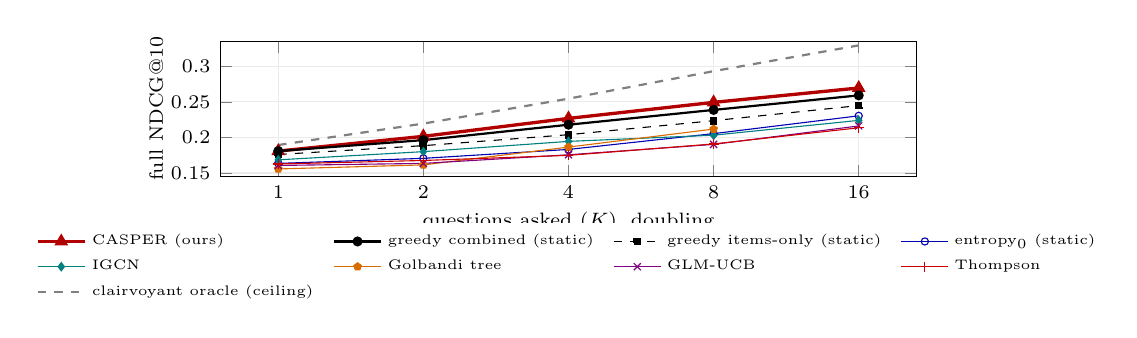
\begin{tikzpicture}
\begin{axis}[
  width=0.86\textwidth, height=3.3cm,
  xmode=log, log basis x=2,
  xtick={1,2,4,8,16}, xticklabels={1,2,4,8,16},
  xlabel={questions asked ($K$), doubling}, ylabel={full NDCG@10},
  ymin=0.145, ymax=0.335,
  grid=major, grid style={black!8},
  tick label style={font=\scriptsize}, label style={font=\scriptsize},
  xlabel style={yshift=2pt}, ylabel style={yshift=-4pt},
  legend style={font=\tiny, at={(0.5,-0.34)}, anchor=north, draw=none,
                /tikz/every even column/.append style={column sep=5pt}},
  legend columns=4,
  legend cell align=left]
\addplot[red!70!black, very thick, mark=triangle*, mark size=1.7] coordinates {(1,.1808)(2,.2015)(4,.2267)(8,.2492)(16,.2694)};
\addlegendentry{CASPER (ours)}
\addplot[black, thick, mark=*, mark size=1.4] coordinates {(1,.1808)(2,.1962)(4,.2178)(8,.2386)(16,.2590)};
\addlegendentry{greedy combined (static)}
\addplot[black, dashed, mark=square*, mark size=1.2] coordinates {(1,.1760)(2,.1884)(4,.2038)(8,.2235)(16,.2447)};
\addlegendentry{greedy items-only (static)}
\addplot[blue!70!black, mark=o, mark size=1.3] coordinates {(1,.1635)(2,.1706)(4,.1831)(8,.2053)(16,.2303)};
\addlegendentry{entropy$_0$ (static)}
\addplot[teal, mark=diamond*, mark size=1.5] coordinates {(1,.1685)(2,.1800)(4,.1944)(8,.2031)(16,.2239)};
\addlegendentry{IGCN}
\addplot[orange!85!black, mark=pentagon*, mark size=1.4] coordinates {(1,.1557)(2,.1614)(4,.1864)(8,.2117)};
\addlegendentry{Golbandi tree}
\addplot[violet, mark=x, mark size=1.8] coordinates {(1,.1606)(2,.1635)(4,.1756)(8,.1902)(16,.2161)};
\addlegendentry{GLM-UCB}
\addplot[red!80!black, mark=+, mark size=1.8] coordinates {(1,.1627)(2,.1676)(4,.1748)(8,.1908)(16,.2135)};
\addlegendentry{Thompson}
\addplot[gray, dashed, thick, mark=none] coordinates {(1,.1893)(2,.2194)(4,.2544)(8,.2930)(16,.3292)};
\addlegendentry{clairvoyant oracle (ceiling)}
\end{axis}
\end{tikzpicture}}
\caption{Full NDCG@10 against question budget, 10{,}000 test users. Budgets double, so the axis is
spaced by powers of two and carries no interpolation between the measured points. The
metric-optimised static orders (black) bound every published selector at every budget; CASPER (red)
is the only arm above them; the oracle (grey), which reads the user's own ratings at selection time,
is a ceiling.}
\label{fig:budget}
\end{figure}

\paragraph{Every published method lands below the fixed order.}
At sixteen questions the greedy items-only sequence reaches $.2447/.1017$, against $.2303/.0924$ for
the entropy$_0$ heuristic~\cite{rashid2008learning} and $.2161/.0833$ for GLM-UCB. The strongest items-only static order leads the best adaptive selector
by $.0281^\star$ $[.0247,.0314]$ full and $.0178^\star$ $[.0145,.0210]$ tail, twice that selector's deficit
against the heuristic. Widened to every adaptive arm, 138 cells in all, the combined and concepts-only orders lead and
separate in all 138 and the items-only order in 136, the exceptions being tail cells separating
neither way.

\paragraph{Tuning the bandits does not change the verdict.}
At the constants chosen on validation, GLM-UCB reaches $.2234/.0841$ at sixteen questions and
Thompson $.2158/.0881$, worth $+.0073$ and $+.0023$ full over their published values and still
$-.0356^\star$ and $-.0432^\star$ below the combined static order ($-.0213$ and $-.0289$ below the
items-only order, the correct comparator for an item-only selector).

\paragraph{The loss is not a failure to branch.}
Thompson sampling conducts a distinct interview for every one of the 10{,}000 users from the fourth
question onward and still loses to one order asked of everybody; GLM-UCB reaches 5{,}739 distinct
interviews by the sixteenth. Part of the mechanism is in the answered column: the static order collects 5.52 answers where
Thompson collects 3.39 and the latent-only acquisition 3.84, because criteria preferring high
posterior movement select items almost no user has seen. It is not the whole mechanism, since GLM-UCB collects
5.24 answers, essentially the static rate, and still loses at every budget. Several selectors carrying the adaptive label in Table~\ref{tab:battery}, which records how each
method is described by its own authors, turn out not to condition on answers at all: IGCN is the
global information-gain static order at four questions or fewer, BALD's acquisition is constant under
a homoscedastic linear-Gaussian likelihood, and A-optimal design contains the questions and not the
answers. Twelve of the twenty-three arms are value-free in that sense.

\paragraph{Exactly one rule optimises the reported metric.}
Auditing what each rule maximises gives the plainest explanation. Of the twenty-one distinct
selection rules the battery implements, exactly one optimises held-out ranking quality, and it is our
static order. The published rules maximise information gain about a latent variable~\cite{ma2019eddi}
or a cluster label~\cite{rashid2008learning}, minimise posterior
variance~\cite{houlsby2011bald} or an A-optimality trace~\cite{anava2015budget,sepliarskaia2018spq},
reduce squared error of rating~\cite{golbandi2011adaptive,zhou2011functional} or profile
reconstruction~\cite{kweon2020deep,proissl2024greedyslim}, or maximise a bandit
index~\cite{zhao2013interactive,zhang2020conucb,wang2023conlinucb,liu2025clisk,parapar2021dpe}.
Optimising a surrogate is not a defect in itself, but six of the thirteen claimed a ranking
improvement on a held-out ranking metric, so holding them to NDCG@10 holds them to their own headline.

\paragraph{Robustness.}
The ordering repeats on RecVAE~\cite{ren2020recvae}, TaNP~\cite{lin2021tanp} and EDDI's
Partial-VAE~\cite{ma2019eddi}, and reverses on one, Golbandi's leaf model, where Thompson sampling
beats the static order at every budget it runs at; Section~\ref{sec:rq3} returns to that consumer
with the absolute numbers.

\paragraph{Answer to RQ1.}
Under one contract, no published selector of any kind beats a fixed order chosen by greedy
maximisation of the reported metric at any budget, and the failure is not a failure to branch.

\section{RQ2: How Far the Surrogates Sit From the Metric}
\label{sec:rq2}

\paragraph{Criterion regret at real states.}
At every node it visits, the tree of Section~\ref{sec:rq3} persists the exact measured cohort-mean
NDCG@10 gain of every candidate over that node's own users: 22 nodes by roughly 1{,}000 candidates of
ground truth for the quantity each criterion approximates. We score three against it
(Table~\ref{tab:criterion}): Golbandi's within-node rating variance~\cite{golbandi2011adaptive}, Hu
and Yu's pairwise rank loss~\cite{hu2013interview}, and the logistic loss their experiments ran.

\begin{table}[tbp]
\centering
\caption{Published split criteria against exact measured NDCG@10 gains at all 22 nodes of the grown
tree. Argmax hit counts nodes where the criterion's top choice is the metric's; top-10 recall is the
mean fraction of the metric's ten best questions that the criterion also ranks in its ten best.
Regret is the user-weighted NDCG@10 forgone by following that criterion instead of the metric;
the last row is the control a criterion must beat. Bold is best of the three criteria.}
\label{tab:criterion}
\small
\begin{tabular}{lrrrrr}
\toprule
criterion & mean $\rho$ & nodes $\rho{>}0$ & argmax hit & top-10 recall & regret \\
\midrule
variance~\cite{golbandi2011adaptive} & $\mathbf{+0.010}$ & \textbf{13/22} & \textbf{1/22} & \textbf{0.03} & $+0.01664$ \\
pairwise rank loss~\cite{hu2013interview} & $-0.060$ & 10/22 & 0/22 & 0.01 & $+0.01738$ \\
logistic loss~\cite{hu2013interview} & $-0.104$ & 9/22 & \textbf{1/22} & \textbf{0.03} & $\mathbf{+0.01282}$ \\
\midrule
\emph{control: uniform random pick} & --- & --- & --- & 0.10 & $+0.01955$ \\
\bottomrule
\end{tabular}
\end{table}

Following any of these criteria recovers only $11$--$34\%$ of the NDCG@10 that a uniformly random
pick leaves unrealised. The rank correlations are approximately zero and two of three are negative,
so these surrogates are not merely weak, two of them point the wrong way: at the states this tree visits they are close to uninformative about
the quantity the field reports, and the pairwise loss selects the measured argmax at no node. At the
root the logistic criterion's argmax is the metric's argmax, while variance ranks that question 250th
of 1{,}000 and the pairwise loss 75th; one level down, no criterion does better than the others. They
agree with the metric where the cohort is largest and stop agreeing where an adaptive method must
earn its keep.

\paragraph{How much is there to adapt to.}
If adaptive selection is to confer a benefit, users must occupy states in which different questions
are optimal. We score each question by $U(q\mid\zz)=\sum_a P(a\mid\zz)\,V(\zz\oplus(q,a))$, with $V$
the expected NDCG@10 of the slate the recommender would show, and report the perplexity of the argmax
distribution: an effective number of distinct optimal questions. Over the concept bank the 10{,}000
cold users share a single one (effective $1.00$); after one standard opener five are optimal
(effective $2.88$), after two, nine (effective $5.04$). Dispersion is not payoff: a policy can manufacture ten thousand distinct
interviews and still lose.

\paragraph{Answer to RQ2.}
The published criteria are close to uninformative about the reported metric at the states an adaptive
interview visits, and after two questions there are roughly five materially different questions to
choose between.

\section{RQ3: Putting the Reported Metric in the Split}
\label{sec:rq3}

RQ1's null and RQ2's diagnosis together specify one experiment. Take the field's own adaptive
machinery, Golbandi's ternary interview tree~\cite{golbandi2011adaptive}, which asks a question at
each node and routes users down a like, dislike or did-not-answer branch, and change exactly one
thing: the scalar by which a candidate question is scored. We call the resulting selector CASPER,
Cold-start Adaptive Selection for Preference Elicitation in Recommendation, a name marking what is
kept, adaptive selection, and what is changed, the quantity selected for. Each of the 1{,}000 candidates, 500
popularity-ranked items and 500 answerability-ranked concepts in one argmax, is scored by the
node-size-weighted mean of its three children's cohort-mean measured held-out full NDCG@10, obtained
by folding that child's answers through the frozen recommender and ranking the catalogue. Nothing is
approximated and no ground truth is read at selection time, since the criterion is a cohort-level
quantity on the validation cohort. The tree is grown there and frozen: depth 5, 15 leaves, 22 nodes,
a minimum leaf size of 200 as the only stopping rule, and sixteen charged questions per user, all
selected by the criterion under test (Table~\ref{tab:tree}). Its root splitter is a concept answered
by $74.2\%$ of the cohort, where the best item split would send 7{,}045 of 10{,}000 users into the
did-not-answer branch. The comparator is a static order built by the same
greedy machinery, on the same objective, pool, candidate mask and cohort, resumed from the tree
root's own search heap, so its first pick is necessarily the tree's root question and the contract
gate is exact: at $K{=}1$ the per-user difference is $0.0$ for all 20{,}000 users.

\begin{table}[tbp]
\centering
\caption{The measured-metric tree against the static order built by the same search on the same
objective, 10{,}000 held-out test users. $K{=}1$ is exactly zero by construction, the contract gate
rather than a result. Absolute at $K{=}16$: tree $0.26936/0.13074$, static $0.25900/0.12370$, no
questions $0.15855/0.02819$. Beyond $K{=}5$ the tree's depth is exhausted and the remaining
questions are chosen inside the reached leaf by the same measured-NDCG search, so the $K{=}16$
gain is five conditioned questions plus a leaf-conditioned tail. Bold is best per column.}
\label{tab:tree}
\small
\begin{tabular}{lcc}
\toprule
$K$ & full gain [95\% CI] & tail gain [95\% CI] \\
\midrule
1 & $0.00000$ (exact) & $0.00000$ (exact) \\
2 & $+0.00528^\star$ $[+0.00324,+0.00725]$ & $-0.00262^\star$ $[-0.00481,-0.00051]$ \\
4 & $+0.00891^\star$ $[+0.00632,+0.01147]$ & $+0.00482^\star$ $[+0.00214,+0.00756]$ \\
8 & $\mathbf{+0.01062}^\star$ $[+0.00775,+0.01354]$ & $\mathbf{+0.00835}^\star$ $[+0.00543,+0.01130]$ \\
16 & $+0.01035^\star$ $[+0.00739,+0.01323]$ & $+0.00705^\star$ $[+0.00394,+0.01012]$ \\
\bottomrule
\end{tabular}
\end{table}

\paragraph{The result, with its qualifier attached.}
Conditioning on cold, closed, charged questions beats a strong static order on held-out users from
four questions onward, on both axes (Table~\ref{tab:tree}); seven of the eight $K\ge2$ intervals
exclude zero in the tree's favour and the eighth, tail at two questions, excludes zero against it.

\paragraph{One variable changed.}
The mechanism claim is about one variable, so we vary that one
(Table~\ref{tab:splitcrit}): same tree code, branch rule, minimum leaf size, charged answers,
recommender, candidate mask, pool, cohorts and budget, with the split criterion replaced by each
published alternative in turn, each scored through its own second-order split gain with nothing
sampled (the pairwise loss sums over all $137{,}591{,}707$ fold-in pairs). Two shuffle controls
complete the set, a uniform draw over the pool and one restricted to candidates whose split clears
the minimum leaf size, the latter the fair control since it destroys only the choice of question.

\begin{table}[tbp]
\centering
\caption{One variable changed: gain against the same static order, 10{,}000 test users, $K{=}16$. All
56 non-nested intervals in the six-arm matrix exclude zero except the pairwise-versus-variance
contrast reported in the text. Bold is best per column.}
\label{tab:splitcrit}
\small
\begin{tabular}{lrrrr}
\toprule
split criterion & full@10 & full gain & tail@10 & tail gain \\
\midrule
measured NDCG@10 (ours) & $\mathbf{0.26936}$ & $\mathbf{+0.01035}^\star$ & $\mathbf{0.13074}$ & $\mathbf{+0.00705}^\star$ \\
pairwise rank loss~\cite{hu2013interview} & $0.22859$ & $-0.03041^\star$ & $0.10031$ & $-0.02338^\star$ \\
rating variance~\cite{golbandi2011adaptive} & $0.22840$ & $-0.03061^\star$ & $0.10124$ & $-0.02246^\star$ \\
logistic loss (as run)~\cite{hu2013interview} & $0.17274$ & $-0.08627^\star$ & $0.06817$ & $-0.05552^\star$ \\
\midrule
shuffle, min-leaf-respecting & --- & $-0.04817^\star$ & --- & $-0.03412^\star$ \\
shuffle, unrestricted & --- & $-0.03934^\star$ & --- & $-0.02126^\star$ \\
\bottomrule
\end{tabular}
\end{table}

Exactly one of the six criteria places the adaptive interview above the static order: changing
nothing but the number a question is scored by flips the sign of the conditioning gain. Three
readings follow, and two were not what we pre-registered. First, \emph{the separating axis is measured
versus surrogate, not ranking versus rating}. Hu and Yu's pairwise rank loss and Golbandi's rating
variance are indistinguishable on our metric, $+0.00020$ $[-0.00331,+0.00371]$ full and $-0.00092$
$[-0.00448,+0.00277]$ tail, the only null in the matrix, so upgrading a rating surrogate to a ranking
surrogate bought nothing. Second, \emph{the failure is in the approximation, not in the shape of the
loss}. At the root the measured held-out pairwise rank loss tracks measured NDCG@10 at Spearman
$+0.784$ and forgoes only $+0.00459$, about $29\%$ of what a random pick forgoes, whereas the
Taylor-approximated training-loss version of the same objective correlates at $-0.149$, ranks the
metric's best question 75th of 1{,}000 and forgoes $+0.01473$.
What does the work is measuring the value of asking rather than a training loss over the tree fit.
Third, \emph{depth alone does not indicate conditioning}: the min-leaf-respecting shuffle grows deeper
(7 against 5), wider (27 leaves against 15) and more varied (286 distinct questions against 159) than
the criterion that wins, and still loses by $-0.04817$. The logistic arm is the sharpest single row:
it opens on exactly our question, then degrades monotonically ($-0.00896$, $-0.02777$, $-0.05605$,
$-0.08627$) until its absolute full NDCG@10 falls below its own one-question value, so a criterion can
agree with the metric on the easiest decision and still walk the interview downhill. The ablation is not a
refutation of the published results on their own protocols.

\paragraph{Changing the bank yields more than conditioning does.}
Measured on the same cohort at the same budget, with every order selected under the scoring contract,
enlarging the bank from films to films plus concept questions (tag-level generalisations a user
can answer without having seen any particular film) with no conditioning of any kind is worth
$+0.01430^\star$ $[+0.01124,+0.01739]$ full, $16.6\%$ of the static order's own lift over asking
nothing, against $+0.01035^\star$ for tree conditioning ($10.3\%$). On the tail the ordering is not close, $+0.02199$ against $+0.00705$. If one
thing can be changed, change what the system asks about rather than how it decides what to ask; this
is the strongest qualification of the conditioning result, and it is measured under the same contract. Answerability carries most of the mechanism, though not all of it: the prefix-optimal joint sequence gives concepts ten of sixteen
slots and both of the first two, the tree opens on a concept, and sixteen item questions collect 3.11
answers where sixteen concept questions collect 12.36; at sixteen questions concepts win the tail and
tie on full ($-0.00003$ $[-0.00315,+0.00310]$ full, $+0.01436^\star$ $[+0.01093,+0.01776]$ tail).

\paragraph{What it costs.}
Five qualifiers travel with $+0.01035$. Validation overstates it ($+0.02794$ full on the selection
cohort). Six of the fifteen leaves lose on test, covering $39.3\%$ of the cohort, because a leaf
inherits questions chosen for its parent's cohort. Conditioning does not touch reach: about $14\%$ of
users answer nothing in the first three questions and stay at the no-answer level. The tree diverges
without being shown to route, a pre-registered congruence test being a null, so no routing claim is
made. And it is expensive to build: 37{,}191 seconds per tree against eleven seconds for the Taylor
construction, though serving is a lookup either way.

\paragraph{Who consumes the answers moves the number further than who chooses the questions.}
CASPER's criterion is the metric computed through the recommender that then scores it, so we hand
the same two banked interviews to three further consumers: RecVAE~\cite{ren2020recvae}, a conjugate
belief accumulator over a frozen factorisation, and Golbandi's leaf model~\cite{golbandi2011adaptive},
which matches a cold user to training users sharing their answer pattern. Nothing is regrown or
re-selected, and the certified consumer reproduces Table~\ref{tab:tree} to five decimals. CASPER
beats the static order on three of the four at every budget, all intervals excluding zero ($+0.01035$
on the certified tower, $+0.00161$ on the accumulator at sixteen questions; RecVAE's $+0.04122$ is
measured against a static arm with almost no usable input and counts for direction only); on the leaf
model it wins at two and four questions and reverses at eight ($-0.01375^\star$). Read
Table~\ref{tab:consumers} down its columns and that reversal is an argument for certifying the
consumer: every cell of the certified tower's block sits above every cell of every other block at the
same budget, CASPER there beating the best arm any other consumer reaches by $+0.0270^\star$,
$+0.0410^\star$ and $+0.0391^\star$ at two, four and eight questions. Choosing the consumer is worth
two to four points where choosing the selector is worth one.

\begin{table}[tbp]
\centering
\caption{The same two interviews, three consumers, 10{,}000 test users, full/tail NDCG@10. Only the
model consuming the answers changes; a fourth, a conjugate accumulator, is omitted for space and
gives $+0.00161^\star$ at $K{=}16$. The leaf model has no sixteen-question row: $3^k$ answer patterns
fragment its training cohort beyond depth eight. $K{=}1$ is omitted: both arms ask the same first
question by construction. Consumers are scored with no popularity floor, so one receiving no usable
input scores near zero: RecVAE ingests liked items only, and its low-budget cells are a property of
that input contract rather than of the interview. The answer-free reference $.1626/.0262$ is the
certified tower's.}
\label{tab:consumers}
\footnotesize
\setlength{\tabcolsep}{4pt}
\begin{tabular}{ll rrrr}
\toprule
consumer & interview & $K{=}2$ & $K{=}4$ & $K{=}8$ & $K{=}16$ \\
\midrule
certified tower & CASPER & $\mathbf{.2015}/.0675$ & $\mathbf{.2267/.0905}$ & $\mathbf{.2492/.1117}$ & $\mathbf{.2694/.1307}$ \\
 & static & $.1962/\mathbf{.0701}$ & $.2178/.0857$ & $.2386/.1033$ & $.2590/.1237$ \\
\midrule
Golbandi leaf & CASPER & $.1745/.0393$ & $.1858/.0526$ & $.1964/.0592$ & --- \\
 & static & $.1626/.0262$ & $.1746/.0478$ & $.2101/.0741$ & --- \\
\midrule
RecVAE & CASPER & $.0428/.0152$ & $.1016/.0399$ & $.1265/.0527$ & $.1769/.0764$ \\
 & static & $.0000/.0000$ & $.0662/.0130$ & $.1162/.0317$ & $.1357/.0409$ \\
\bottomrule
\end{tabular}
\end{table}

\paragraph{Answer to RQ3.}
Substituting the reported metric for the published criterion inside the field's own interview tree,
everything else held fixed, reverses the RQ1 comparison from four questions onward on both axes
($+0.01035$ full, $+0.00705$ tail at sixteen) where the published surrogates lose by three times that
margin; changing the question bank with no conditioning is worth more still ($+0.01430$ full,
$+0.02199$ tail).

\section{Limitations and Conclusion}
\label{sec:limits}

Whether a question is answerable is inferred from the same history that scores the user: answer
values are behavioural throughout, and it is the answerability judgement that is a modelling
assumption, standard here and load-bearing for two mechanisms above. A behavioural answer is also one
the user once gave, not one they would give in conversation, and that gap is not measured. Nor are
the channels commensurable per question: a concept answer summarises many films where an item answer
carries one, so that channel's advantage is answerability together with breadth, not answerability
alone. Everything here is one dataset, one split and one seed, on one instrument; the criterion-regret
table in particular would need a second certified recommender to travel. And no published number
validates our comparator, since no prior work has published a static order built by greedily
maximising cohort-mean held-out NDCG@10; the recipe is deterministic, it beats every published
selector we ran, and rebuilding it under the scoring contract cut the conditioning gain from
$+0.01371$ to $+0.01035$, so we have measured what its weakness costs. The fitting asymmetry it
carries is stated and bounded in Section~\ref{sec:contract}.

\medskip\noindent
Put the reported metric into the split criterion and the field's own interview tree rises above a
strong static order ($+0.01035$ at sixteen questions), where five published criteria fitted by the
same search on the same data do not; change what the system asks about rather than how it chooses,
and the gain is larger still ($+0.01430$) with no conditioning at all. The setting is the audit:
thirteen published methods, twenty-three arms, one contract, every one losing to a fixed order built
by greedily maximising the reported metric, none optimising the metric it is judged on. That order
carries a fitting advantage no ported method has, so the audit is a diagnosis, not a ranking. Build the selector around the quantity that will be reported, and
certify its consumer.

\bibliographystyle{splncs04}
\bibliography{refs}

\end{document}
